\documentclass[12pt]{article}
\usepackage[english]{babel}
\usepackage[utf8]{inputenc}

%% Pointer to 'default' preamble, other reusable files
% pacakages and definitions

\usepackage{geometry}
\geometry{
	letterpaper, 
	portrait, 
	top=.75in,
	left=.8in,
	right=.75in,
	bottom=.5in		} 	% Page Margins
	
%% additional packages for nice things
\usepackage{amsmath} 	% for most math
\usepackage{commath} 	% for abs
\usepackage{lastpage}	% for page count
\usepackage{amssymb} 	% for therefore
\usepackage{graphicx} 	% for image handling
\usepackage{wrapfig} 	% wrap figures
\usepackage[none]{hyphenat} % for no hyphenations
\usepackage{array} 		% for >{} column characterisctis
\usepackage{physics} 	% for easier derivative \dv....
\usepackage{tikz} 		% for graphic@!
\usepackage{circuitikz} % for circuits!
\usetikzlibrary{arrows.meta} % for loads
\usepackage[thicklines]{cancel}	% for cancels
\usepackage{xcolor}		% for color cancels
\usepackage[per-mode=fraction]{siunitx} % for si units and num
\sisetup{group-separator = {,}, group-minimum-digits = 3} % additional si unit table functionality

\usepackage{fancyhdr} 	% for header
\usepackage{comment}	% for ability to comment out large sections
\usepackage{multicol}	% for multiple columns using multicols
\usepackage[framed,numbered]{matlab-prettifier} % matlab sytle listing
\usepackage{marvosym} 	% for boltsymbol lightning
\usepackage{pdflscape} 	% for various landscape pages in portrait docs.
%\usepackage{float}
\usepackage{fancyvrb}	% for Verbatim (a tab respecting verbatim)
\usepackage{enumitem}	% for [resume] functionality of enumerate
\usepackage{spreadtab} 	% for using formulas in tables}
\usepackage{numprint}	% for number format in spread tab
\usepackage{subcaption} % for subfigures with captions
\usepackage[normalem]{ulem} % for strike through sout

% for row colors in tables....
\usepackage{color, colortbl}
\definecolor{G1}{gray}{0.9}
\definecolor{G2}{rgb}{1,0.88,1}%{gray}{0.6}
\definecolor{G3}{rgb}{0.88,1,1}

% For table formatting
\usepackage{booktabs}
\renewcommand{\arraystretch}{1.2}
\usepackage{floatrow}
\floatsetup[table]{capposition=top} % put table captions on top of tables

% Caption formating footnotesize ~ 10 pt in a 12 pt document
\usepackage[font={small}]{caption}

%% package config 
\sisetup{output-exponent-marker=\ensuremath{\mathrm{E}}} % for engineer E
\renewcommand{\CancelColor}{\color{red}}	% for color cancels
\lstset{aboveskip=2pt,belowskip=2pt} % for more compact table
%\arraycolsep=1.4pt\def
\setlength{\parindent}{0cm} % Remove indentation from paragraphs
\setlength{\columnsep}{0.5cm}
\lstset{
	style      = Matlab-editor,
	basicstyle = \ttfamily\footnotesize, % if you want to use Courier - not really used?
}
\renewcommand*{\pd}[3][]{\ensuremath{\dfrac{\partial^{#1} #2}{\partial #3}}} % for larger pd fracs
\renewcommand{\real}[1]{\mathbb{R}\left\{ #1 \right\}}	% for REAL symbol
\newcommand{\imag}[1]{\mathbb{I}\left\{ #1 \right\}}	% for IMAG symbol
\definecolor{m}{rgb}{1,0,1}	% for MATLAB matching magenta
	
%% custom macros
\newcommand\numberthis{\addtocounter{equation}{1}\tag{\theequation}} % for simple \numberthis command

\newcommand{\equal}{=} % so circuitikz can have an = in the labels
\newcolumntype{L}[1]{>{\raggedright\let\newline\\\arraybackslash\hspace{0pt}}m{#1}}
\newcolumntype{C}[1]{>{\centering\let\newline\\\arraybackslash\hspace{0pt}}m{#1}}
\newcolumntype{R}[1]{>{\raggedleft\let\newline\\\arraybackslash\hspace{0pt}}m{#1}}

%% Header
\pagestyle{fancy} % for header stuffs
\fancyhf{}
% spacing
\headheight 29 pt
\headsep 6 pt
%%% custom commands for nicer units
\newcommand{\mw}{\ensuremath{\text{ MW}}}
\newcommand{\hz}{\ensuremath{\text{ Hz}}}
\newcommand{\pu}{\ensuremath{\text{ Pu}}}
\newcommand{\sbase}{\ensuremath{\text{S}_{\text{Base}}}}
\newcommand{\fbase}{\ensuremath{f_{\text{Base}}}}
\newcommand{\mbase}[1]{\ensuremath{\text{M}_{\text{Base}_{#1}}}}
\newcommand{\hsys}{\ensuremath{\text{ H}_{\text{sys}}}}


%% Header
\rhead{Thad Haines \\ Page \thepage\ of \pageref{LastPage}}
\chead{Talking Points \\ Week of July 1st, 2019}
\lhead{Research \\ }

\begin{document}
\begin{multicols}{2}
\raggedright
	\paragraph{Recent Progress:}
	\begin{enumerate}

		\item \textbf{PSLF License Renewed}.
		\item 2 weeks left on contract.
		\item Balancing Authority ACE filtering expanded.
		\item Six Machine Trip Testing.
		\item MiniWECC Step and Trip Testing.
		

	%	\item More \verb|matplotlib| plot functions created.

		\item GitHub updated:\\
		\verb|https://github.com/thadhaines/|
		
	\end{enumerate}
\paragraph{Current Tasks:}
	\begin{enumerate}

		\item Continue to Update Code flowchart to aid in further development.
		\item Bring wind into simulation.
		\item Work to incorporate Matt's \emph{Suggested Use Cases} into simulation.
		\begin{itemize}
		
		\item Add Shunt Group Agent
		\item Work to Define Definite Time Controller user input
		
		\item Continue to Refine BA ACE actions.

		\end{itemize}
		%\item Keep Goals and Requests in mind.
		
		%\subitem A FlowtabrDAO exists that can find flow between busses. A way to initialize bus connections between areas has yet to be devised.

	\end{enumerate}

	\paragraph{Current Questions:}
	\begin{enumerate}
	
	\item Best way to trip generators on/off in PSDS?
	\item Could improper tripping cause non-convergence?
	
	\item \sout{Could exciters be responsible for initial voltage differences in MiniWECC tests?} (resolved)

	\item What is the end goal of this research?
	\subitem Long-term simulation of governor and AGC interaction to wind ramps while controlling voltage stability via logic controlled switchable shunts.
	
	 Simulation uses large time steps, ignores inter-machine oscillations, utilizes a time sequence of power flows for system bus states, a single aggregate swing equation for frequency, and reduces governor models to 2nd order. (?)
	
	%	\item Overview of planned PSLF scenarios? $\rightarrow$ Similar to Heredia paper but on Wecc/MiniWecc Scale? 
		
	%	\item Is there more available/relevant event data that may help us to verify simulations of specific instances (wind ramps or other behavior) that novel research will focus on? %(Heredia paper data helpful for some wind ramp data context)

	%	\item  Any progress / continued interest in miniWecc Area definitions?


\vfill\null
\columnbreak

\paragraph{Future Tasks:} %(Little to No Progress since last time / Things coming down the pipe)
	\begin{enumerate}

		\item Account for different types of loads (exponential load model)
		
		\item Formulate feasible plan of action for casting all WECC governors to LTD governors (tgov1). Something like:
		\begin{enumerate}
		\item Parse models of interest from dyd.
		\item Create dyd from parsed model.
		\item Automate a 'scaled' Pref step test for a one machine infinite bus in PSDS.
		\item Read and analyze output data
		\item Generate/Calculate LTD equivalent model parameters from results (this will probably use MATLAB and \verb|jfind|)
		\item Export custom dyd for LTD simulation. (PSDS would still use original the dyd, though \emph{could} use modified dyd)
		\end{enumerate}

		\item Add import mirror / bypass mirror init sequence option to prevent repeated mirror creations.

		\item Create an agent for every object: \\ ULTC, SVD, Transformer, \ldots
		
		\item Investigate line current data and ULTC action in PSDS.
		
	\end{enumerate}

\paragraph{Matt Requests:}
\begin{enumerate}
		\item Enable multiple dyd files to overwrite / replace previously defined agents/parameters
		\item Allow for variable time steps.
\end{enumerate}

	\end{enumerate}
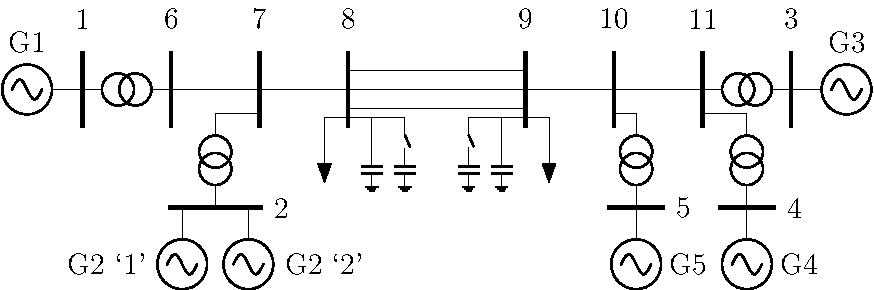
\includegraphics[width=\linewidth]{../../models/sixMachine/sixMachine}

%\paragraph{'Soft Goals':}
%	\begin{enumerate}
%	\item Write Thesis 2020
%	\end{enumerate}
		

\vfill\null

\end{multicols}

\pagebreak
\paragraph{ACE Conventions:} Positive ACE denotes over generation. $B$ (the frequency bias) is negative.
\begin{align*}
\text{ACE}_{\text{tie line}} &= P_{gen} - P_{load} - P_{\text{sched interchange}}\\
\text{ACE}_{\text{frequency bias}} &= 10B(f_{\text{actual}}-f_{\text{sched}})f_{base}\\
\text{ACE} &= \text{ACE}_{\text{tie line}} -\text{ACE}_{\text{frequency bias}}
\end{align*}
\paragraph{Final ACE Results:} Event is a 75 MW load step in Area 2 of Six Machine System.\\

\begin{minipage}{\linewidth}
		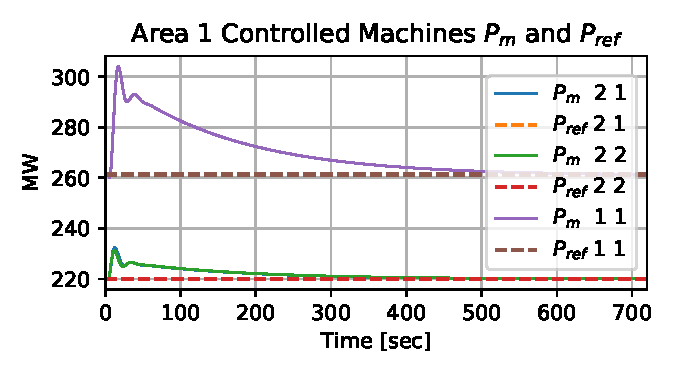
\includegraphics[width=.5\linewidth]{SixMachineStepBA4BA1}
		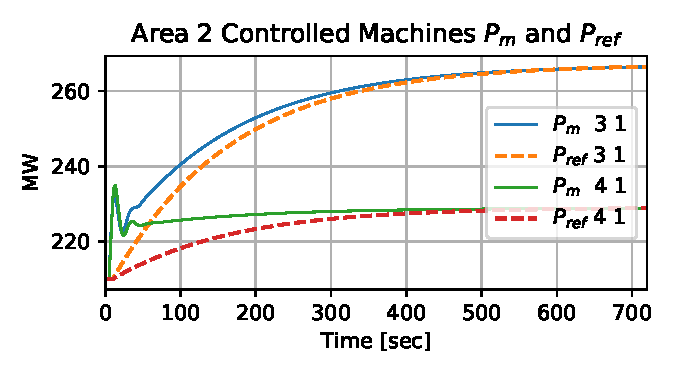
\includegraphics[width=.5\linewidth]{SixMachineStepBA4BA2}
\end{minipage}
\begin{minipage}{\linewidth}
		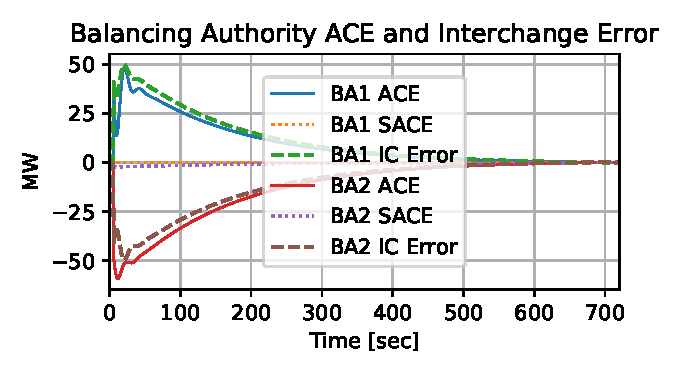
\includegraphics[width=.5\linewidth]{SixMachineStepBA4ACE}
		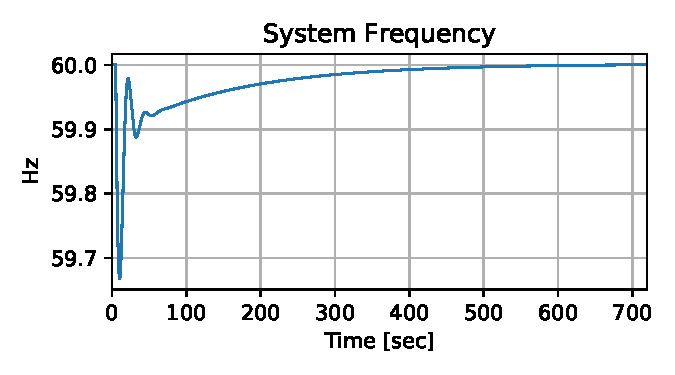
\includegraphics[width=.5\linewidth]{SixMachineStepBA4Freq}
\end{minipage}

\paragraph{MiniWECC Gen Trip:} Tripping Gen 27 (212.5 MW) at t=2. \\
Theoretical SS calculation requires tripped generator MW and change in system losses.
\begin{figure}[h!]
		\centering
		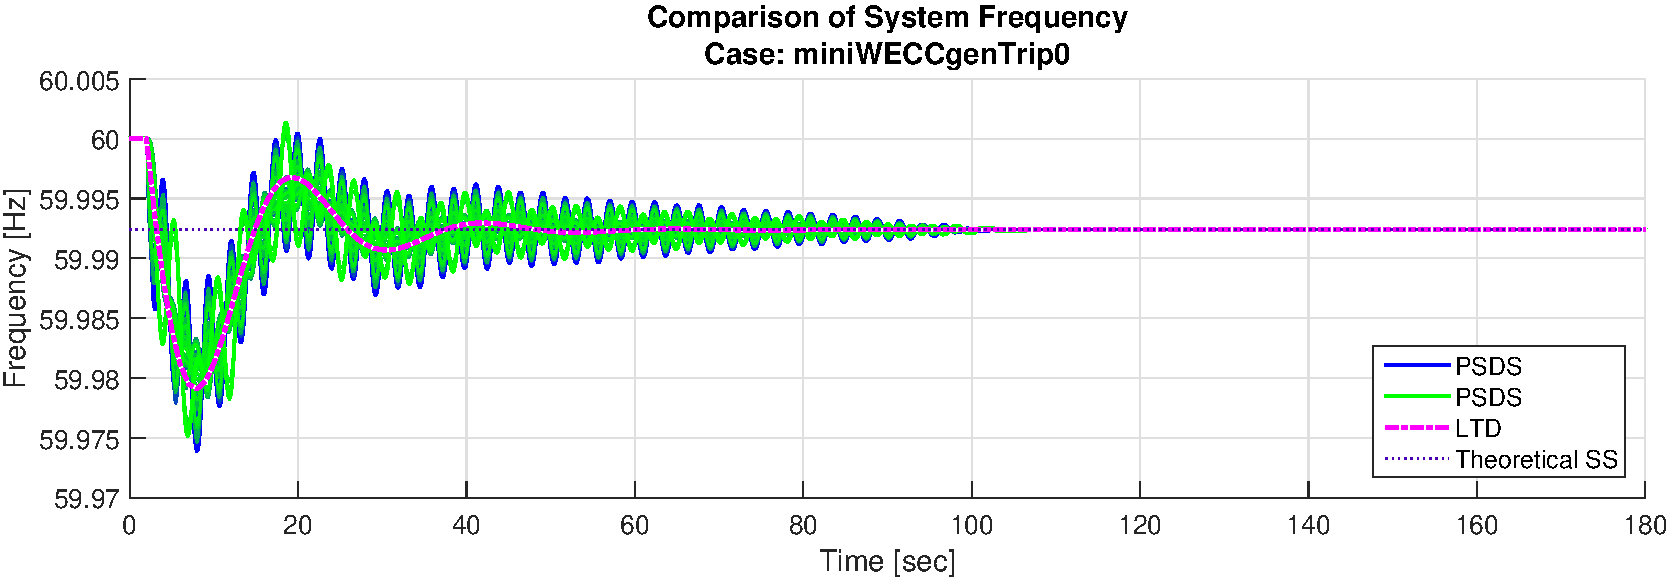
\includegraphics[width=\linewidth]{../../one_offs/miniWECC_v02/miniWECCgenTrip0Freq}\vspace{-1em}
		%\caption{Generator Electrical Power Output}
		%\label{ Pe}		 
\end{figure}

Tripping other generators (colstrip) causes Python run PSLF load flow solution to diverge. \\
The PSDS simulation does not crash during similar events.\\
The PSLF load flow does not diverge if the same generator is set to St=0 from PSLF.\\
Voltage magnitudes and angles from LTD do not match PSDS.
\end{document}